\documentclass[
    a4paper,
    12pt,
    titlepage,
    bibliography=totoc,
    twoside=on,
    parskip=false,
    numbers=noenddot,
    cleardoublepage=empty,
    DIV=12,
    BCOR=12.0mm,
    headheight=36pt,
    headings=openright
]{scrreprt}

\raggedbottom

\usepackage[utf8]{inputenc}
\usepackage[T1]{fontenc}
\usepackage{lmodern}
\usepackage[english,ngerman]{babel}
\usepackage[automark,headsepline]{scrlayer-scrpage}
\usepackage{setspace}
\onehalfspacing
\KOMAoptions{DIV=last}

\usepackage{csquotes}
\usepackage[backend=biber,style=numeric,sorting=none,maxbibnames=99]{biblatex}
\addbibresource{diss_bib.bib}

\usepackage[labelfont=bf]{caption}
\usepackage{subcaption}
\usepackage{graphicx}
\graphicspath{{pictures/}}
\usepackage{xcolor}
\usepackage[section]{placeins}
\usepackage{float}
\usepackage{booktabs}
\usepackage{tabularx}
\usepackage{array}
\usepackage{enumitem}
\usepackage{amsmath,amssymb}
\usepackage[locale=DE]{siunitx}
\usepackage{tikz}
\usetikzlibrary{arrows.meta,positioning,shapes.geometric,fit,backgrounds}
\usepackage{xstring}
\usepackage[bookmarksnumbered=true]{hyperref}

\definecolor{turot}{RGB}{197,14,31}
\definecolor{tublau}{RGB}{0,166,179}
\definecolor{tugrau}{RGB}{113,113,113}
\definecolor{tugelb}{RGB}{255,128,0}
\definecolor{tugruen}{RGB}{34,161,92}

\hypersetup{
  colorlinks=true,
  urlcolor=black,
  citecolor=black,
  linkcolor=black,
  pdfstartview=Fit,
  pdftitle={Deployment-Oriented Artificial Intelligence for Battery Management Systems},
  pdfauthor={Florian Rzepka, Technische Universitaet Berlin},
  pdfsubject={Working dissertation structure},
  pdfkeywords={battery management system, embedded AI, state estimation, dissertation}
}

\newcolumntype{Y}{>{\raggedright\arraybackslash}X}

\newcommand{\chapterrole}[1]{%
    \begin{quote}
    \textbf{Role in the dissertation.} #1
    \end{quote}
}

\newcommand{\placeholderfigure}[2]{%
    \begin{figure}[H]
        \centering
        \fbox{%
            \parbox{0.86\textwidth}{%
                \textbf{Planned figure placeholder}\\[3pt]
                #1
            }%
        }
        \caption{#2}
    \end{figure}
}

\setkomafont{chapter}{\Huge}
\setkomafont{chapterprefix}{\large}
\newkomafont{chapternumber}{\mdseries\fontsize{50pt}{60pt}\selectfont}
\renewcommand\raggedchapter{\raggedleft}

\tikzset{
    headings/base/.style={
        outer sep=0pt,
        inner sep=5pt,
    },
    headings/chapterbackground/.style={
        headings/base,
        shade,
        left color=white,
        right color=white,
    },
    headings/chapapp/.style={
        headings/base,
        text=tugrau,
        font=\usekomafont{chapterprefix}
    },
    headings/chapternumber/.style={
        headings/base,
        text=tugrau,
        font=\usekomafont{chapternumber}
    },
    headings/chapterline/.style={
        tugrau,
        line width=2pt
    }
}

\makeatletter
\renewcommand*\chapterlinesformat[3]{%
  \Ifstr{#1}{chapter}{%
    \begin{tikzpicture}[baseline=(title.base)]
      \node[headings/chapterbackground](title){%
        \parbox[t]{\dimexpr\textwidth-2\pgfkeysvalueof{/pgf/inner xsep}\relax}{\raggedchapter #3}%
      };
      \node[headings/chapapp,anchor=south east]
        at (title.north east){\Ifstr{#2}{}{}{\chapapp}\strut};
      \useasboundingbox
        (current bounding box.north west)
        rectangle
        ([yshift=-10pt]current bounding box.south east);
      \draw[headings/chapterline]
        (current bounding box.south east)++(+.5\pgflinewidth,0)--+(0,\paperheight);
      \node[anchor=base west,headings/chapternumber]
        at([xshift=10pt]title.base-|current bounding box.east){#2};
    \end{tikzpicture}
    \par
  }{%
    \@hangfrom{#2}{#3}%
  }%
}
\makeatother

\pagestyle{scrheadings}
\automark[section]{chapter}
\ihead[]{}
\chead[]{}
\ohead[]{\headmark}
\ifoot[]{}
\cfoot[]{}
\ofoot[\thepage]{\thepage}

\begin{document}
\pagenumbering{Roman}

\begin{titlepage}
\thispagestyle{empty}
\begin{singlespace}
\begin{center}
\vspace*{15pt}
\begin{onehalfspace}
\Huge{\textbf{Deployment-Oriented Artificial Intelligence}}\\
\vspace*{10pt}
\Large{\textbf{for Battery Management Systems}}\\
\vspace*{10pt}
\Large{\textbf{Neural network ageing estimation, robustness benchmarking,}}\\
\Large{\textbf{embedded optimization, and hardware integration}}
\end{onehalfspace}
\vspace*{30pt}
\large{vorgelegt von\\
M. Sc.\\
Florian Rzepka\\
geb. in Berlin}\\
\vspace*{40pt}

\large{
von der Fakult\"at IV -- Elektrotechnik und Informatik\\
der Technischen Universit\"at Berlin\\
zur Erlangung des akademischen Grades\\}
\vspace{17pt}

\large{
Doktor der Ingenieurwissenschaften\\
-- Dr.-Ing. --\\
}

\vspace{12pt}
\large{Arbeitsfassung zur Strukturierung der Dissertation\\}
\end{center}

\vspace{36pt}
\begin{flushleft}
\large{Promotionsausschuss:\\}
\large{Vorsitzende*r: tbd\\
Gutachter*in: tbd\\
Gutachter*in: tbd\\
}
\vspace{10pt}
\large{Tag der wissenschaftlichen Aussprache: tbd\\}
\end{flushleft}
\vspace{10pt}
\begin{center}
\large{Berlin, 2026}
\end{center}
\end{singlespace}
\end{titlepage}

\cleardoublepage
\chapter*{Vorwort}
\addcontentsline{toc}{chapter}{Vorwort}
This document is a working dissertation mockup. Its purpose is not to provide final prose yet, but to establish a coherent overall narrative, a plausible chapter order, and a first impression of how the dissertation could look when the existing and planned papers are integrated into one thesis manuscript.

\chapter*{Abstract}
\addcontentsline{toc}{chapter}{Abstract}
This dissertation is structured around the deployment-oriented development of artificial intelligence for battery management systems. The planned narrative begins with neural-network-based ageing estimation for stationary storage systems, continues with robustness benchmarking of embedded battery state estimation under disturbed measurements, and then moves toward embedded implementation on microcontrollers using pruning and quantization. A further planned component studies how compression methods interact with different model architectures, while an additional hardware chapter documents the custom battery management system platform and the practical route from algorithm development to embedded execution. The central idea of the dissertation is that battery intelligence should be evaluated not only by nominal prediction accuracy, but by the combined requirement space of estimator performance, hardware feasibility, and implementation effort.

\chapter*{Kurzzusammenfassung}
\addcontentsline{toc}{chapter}{Kurzzusammenfassung}
Die Dissertation wird als durchgehende, anwendungsorientierte Geschichte f\"ur k\"unstliche Intelligenz im Batteriemanagement aufgebaut. Im Mittelpunkt stehen erstens neuronale Architekturen zur Alterungsbestimmung station\"arer Speichersysteme, zweitens die Robustheit eingebetteter Zustandsbestimmung unter realistischen Messst\"orungen, drittens die effiziente Ausf\"uhrung solcher Modelle auf Mikrocontrollern durch Pruning und Quantisierung sowie viertens die Einbettung in eine reale Hardware- und BMS-Plattform. Die \"ubergeordnete Leitidee ist, dass KI-gest\"utzte BMS-Methoden nicht nur nach Genauigkeit, sondern entlang der drei Anforderungsfelder Leistung, Hardware und Implementierungsaufwand bewertet werden sollten.

\tableofcontents
\cleardoublepage

\chapter*{Abbreviations}
\addcontentsline{toc}{chapter}{Abbreviations}
\begin{description}[style=nextline,leftmargin=3cm]
\item[AI] Artificial Intelligence
\item[BMS] Battery Management System
\item[ECM] Equivalent Circuit Model
\item[LSTM] Long Short-Term Memory
\item[MCU] Microcontroller Unit
\item[MLP] Multilayer Perceptron
\item[SOC] State of Charge
\item[SOH] State of Health
\end{description}

\chapter*{Symbols}
\addcontentsline{toc}{chapter}{Symbols}
\begin{description}[style=nextline,leftmargin=3cm]
\item[$SOC$] State of charge
\item[$SOH$] State of health
\item[$Q$] Cumulative charge or charge throughput
\item[$t$] Time
\item[$U$] Voltage
\item[$I$] Current
\end{description}

\listoffigures
\addcontentsline{toc}{chapter}{List of Figures}
\listoftables
\addcontentsline{toc}{chapter}{List of Tables}

\cleardoublepage
\pagenumbering{arabic}

\chapter{Introduction and Motivation}
\chapterrole{This opening chapter should make clear that the dissertation is not a loose bundle of papers. It should define a single scientific story: how battery intelligence moves from data-driven ageing estimation toward robust and resource-efficient embedded deployment inside practical BMS environments.}

The overarching motivation of the dissertation is the gap between algorithm-centric battery AI research and deployable BMS intelligence. In many papers, the central question is still whether a model reaches a low error on a clean dataset. In a deployable battery system, however, the more relevant question is whether the method remains useful when it must run on constrained hardware, tolerate imperfect measurements, and fit into a real engineering workflow. This dissertation therefore places prediction quality, robustness, embedded feasibility, and hardware integration into one combined research frame.

\section{Central Thesis}
The central thesis of the dissertation is that AI-enabled BMS functions should be designed and evaluated along three linked requirement dimensions:
\begin{itemize}[leftmargin=*]
\item estimator performance, including baseline accuracy, recovery behavior, and robustness against realistic disturbances,
\item hardware feasibility, including microcontroller resources, latency, integration constraints, and measurement-chain limitations,
\item implementation strategy, including feature engineering, model architecture, compression, and the route from research code to embedded inference.
\end{itemize}

\section{Research Questions}
\begin{enumerate}[leftmargin=*]
\item How can neural-network architectures represent battery ageing in stationary storage systems with sufficient interpretability and practical utility?
\item How do embedded battery state estimators behave when realistic measurement disturbances and timing irregularities are introduced?
\item How can AI-based SOC and SOH estimators be reduced and transferred onto microcontrollers without losing too much predictive utility?
\item How strongly does the effect of quantization and pruning depend on the underlying model architecture?
\item How should a hardware platform and validation chain be structured so that AI-based BMS methods can be tested under realistic embedded conditions?
\end{enumerate}

\section{Included and Planned Publications}
The dissertation integrates the published and planned work listed in Table~\ref{tab:publication_map}. The intended narrative order follows your preferred logic: first the ageing-estimation work, then the robustness benchmark, then the embedded deployment paper, followed by the planned compression study and the hardware-focused integration perspective.\autocite{paper1_soh,paper3_robustness,paper2_embedded,paper4_planned}

\begin{table}[H]
    \centering
    \caption{Mapping of the included and planned work to the dissertation narrative.}
    \label{tab:publication_map}
    \begin{tabularx}{\textwidth}{p{1.8cm}p{5.3cm}p{2.7cm}Y}
        \toprule
        Order & Source work & Primary dimension & Intended role in the dissertation \\
        \midrule
        1 & Neural Network Architecture for Determining the Aging of Stationary Storage Systems in Smart Grids & Model design and ageing estimation & Establishes the data-driven ageing-estimation foundation and motivates the role of feature engineering, temporal context, and model architecture. \\
        2 & Performance Benchmarking of Embedded Battery State Estimation & Robustness and deployment-facing performance & Introduces the dissertation-wide requirement space and shows why clean-condition accuracy alone is insufficient. \\
        3 & Embedded Artificial Intelligence in Battery Management Systems & Embedded deployment and optimization & Connects model design to actual MCU execution through pruning, quantization, latency, and memory metrics. \\
        4 & Planned comparative study on pruning and quantization across architectures & Compression sensitivity and co-design & Extends the embedded perspective from one concrete pipeline toward a broader architecture-dependent design framework. \\
        5 & Planned hardware integration chapter around the custom BMS platform & Hardware and validation ecosystem & Anchors the software and model contributions in a real system context and test environment. \\
        \bottomrule
    \end{tabularx}
\end{table}

\begin{figure}[H]
    \centering
    \begin{tikzpicture}[
        >=Latex,
        topic/.style={draw=tublau, rounded corners=4pt, fill=tublau!10, text width=4.1cm, align=left, inner sep=8pt},
        base/.style={draw=tugrau, rounded corners=4pt, fill=tugrau!12, text width=14.0cm, align=left, inner sep=8pt},
        synth/.style={draw=tugruen, rounded corners=4pt, fill=tugruen!12, text width=14.0cm, align=left, inner sep=8pt}
    ]
        \node[base] (foundation) at (0,0) {\textbf{Foundation layer:} datasets, ageing experiments, embedded targets, and the custom BMS / validation ecosystem.};
        \node[topic] (p1) at (-6.2,2.8) {\textbf{Chapter 5}\\Paper 1\\Neural ageing estimation for stationary storage};
        \node[topic] (p3) at (-2.0,2.8) {\textbf{Chapter 6}\\Paper 3\\Robustness benchmark for embedded state estimation};
        \node[topic] (p2) at (2.2,2.8) {\textbf{Chapter 7}\\Paper 2\\Pruning and quantization for MCU deployment};
        \node[topic] (p4) at (6.4,2.8) {\textbf{Chapter 8}\\Planned paper\\Compression study across architectures};
        \node[synth] (synthesis) at (0,5.6) {\textbf{Synthesis layer:} deployment-oriented design rules for BMS intelligence across performance, hardware, and implementation.};
        \draw[->,thick] (foundation.north west) ++(2.0,0) -- (p1.south);
        \draw[->,thick] (foundation.north west) ++(6.2,0) -- (p3.south);
        \draw[->,thick] (foundation.north east) ++(-6.2,0) -- (p2.south);
        \draw[->,thick] (foundation.north east) ++(-2.0,0) -- (p4.south);
        \draw[->,thick] (p1.north) -- (synthesis.south west);
        \draw[->,thick] (p3.north) -- (synthesis.south west);
        \draw[->,thick] (p2.north) -- (synthesis.south east);
        \draw[->,thick] (p4.north) -- (synthesis.south east);
    \end{tikzpicture}
    \caption{Proposed dissertation roadmap. The existing papers form the main argumentative chain, while the hardware ecosystem and the planned compression study widen the work from algorithmic performance toward full deployment-oriented BMS intelligence.}
    \label{fig:diss_roadmap}
\end{figure}

\chapter{Dissertation Framework and Requirement Space}
\chapterrole{This chapter should introduce the conceptual frame that ties the dissertation together. The requirements graphic from the robustness paper is well suited to become the central figure of the entire thesis.}

The strongest unifying concept already available in the current paper set is the requirement-space view from the robustness benchmark. It separates deployment-oriented battery intelligence into performance, hardware, and implementation considerations. This figure is therefore a natural candidate for the dissertation-wide framing chapter, because it prevents the thesis from being read as a simple succession of disconnected paper topics.

\begin{figure}[H]
    \centering
    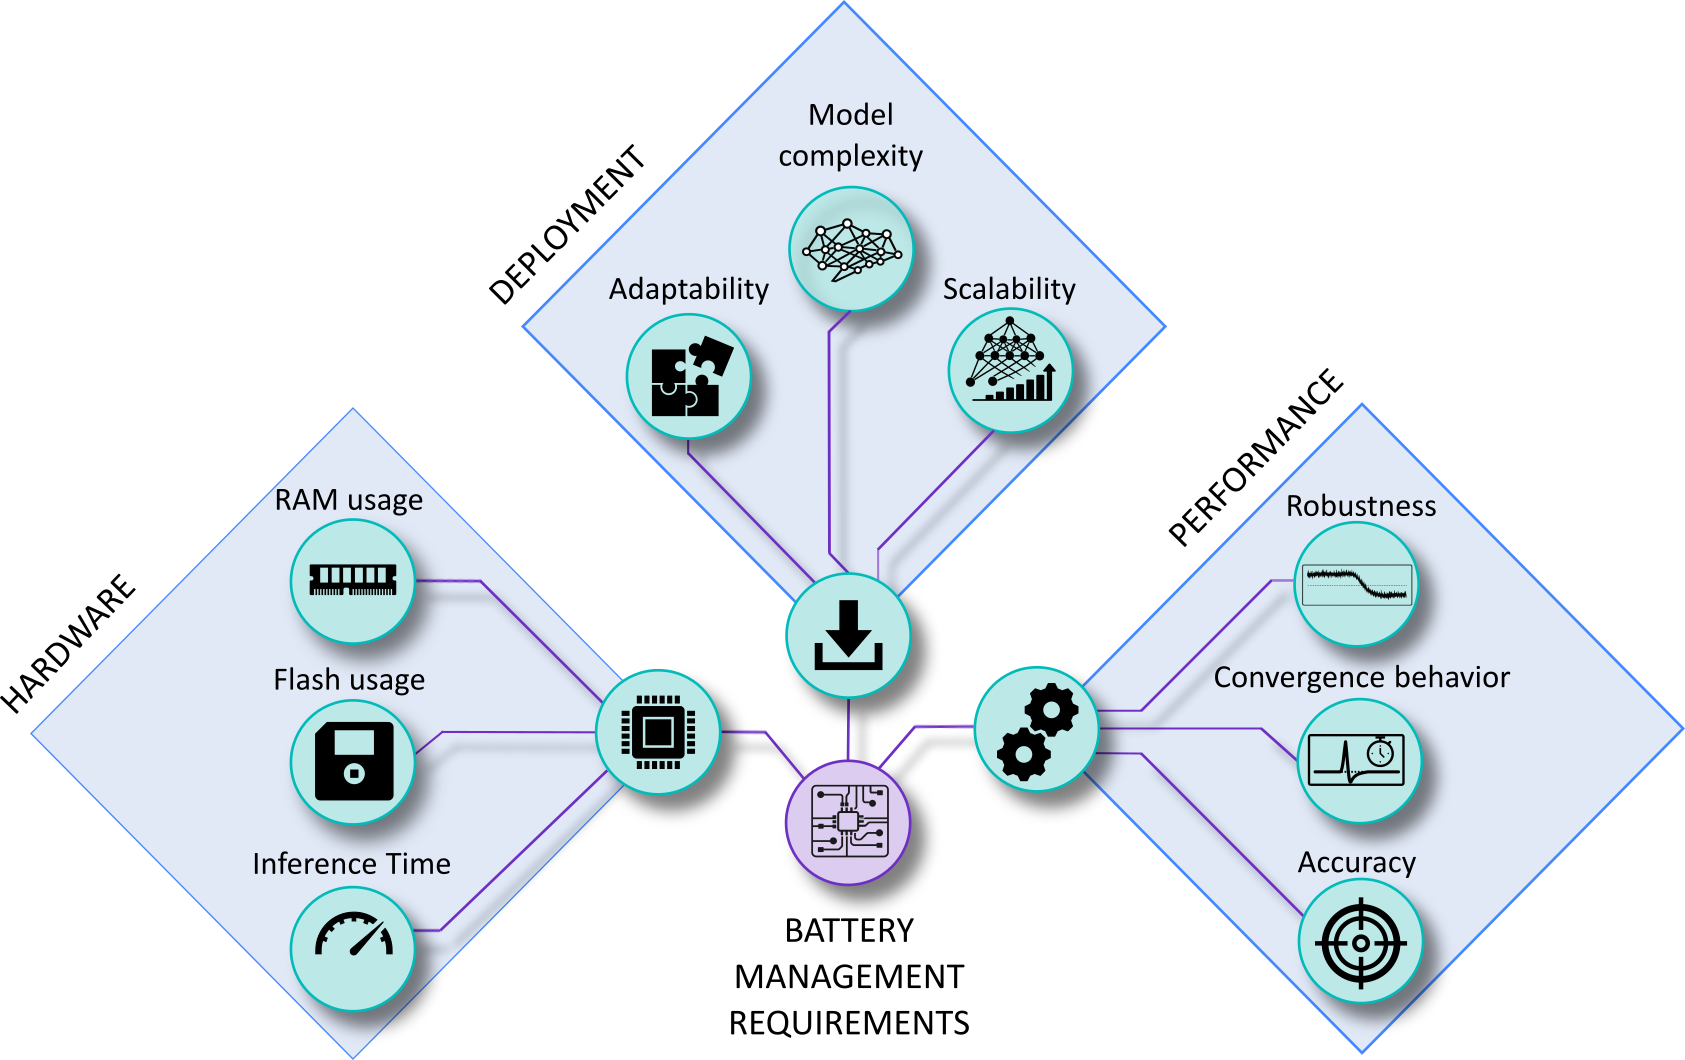
\includegraphics[width=0.92\textwidth]{bms_requirements.png}
    \caption{Working dissertation framing based on the requirement-space figure from the robustness benchmark. In the dissertation, this figure can be reinterpreted as the global structure that connects algorithm design, embedded feasibility, and hardware integration.}
    \label{fig:bms_requirements}
\end{figure}

\section{Performance Dimension}
This dimension captures nominal estimator quality, robustness under disturbed measurements, and synchronization behavior after mismatched initial conditions or missing data. It is primarily represented by the robustness benchmark chapter, but it should also be used as a lens for interpreting the embedded and ageing-estimation chapters.

\section{Hardware Dimension}
This dimension captures what the algorithm must respect once it is placed into a BMS setting: sensing, memory, computation time, microcontroller capabilities, and the practical route toward a testable prototype. This dimension justifies the later chapters on MCU execution and the custom BMS platform.

\section{Implementation Dimension}
This dimension captures how the method is actually built: architecture choice, temporal context, feature engineering, compression strategy, and software-to-firmware transfer. It links the SOH architecture work, the embedded AI work, and the planned cross-architecture compression study.

\section{How the Thesis Should Read as One Story}
The dissertation should not be organized around journals or submission histories. Instead, it should read from left to right through the requirement space:
\begin{itemize}[leftmargin=*]
\item first, how a neural model can capture ageing information in the battery domain,
\item second, why estimator quality must be judged under realistic disturbances,
\item third, how the resulting models can be translated into efficient embedded inference,
\item fourth, how a real hardware ecosystem can host, validate, and extend such methods.
\end{itemize}

\chapter{State of the Art and Technical Background}
\chapterrole{This chapter should provide the common vocabulary for all later chapters and prevent repeated background sections inside the integrated paper material.}

\section{Battery Management Systems}
This section should introduce battery-system functions, the role of the BMS, and the relation between sensing, control, safety, and diagnosis. It should define how SOC and SOH support energy management, operating limits, charging strategies, and lifetime-aware operation.

\section{Neural Networks for Battery Ageing and State Estimation}
This section should summarize why neural methods are attractive in battery applications: nonlinear representation power, temporal modeling, data-driven feature fusion, and the flexibility to capture ageing-related patterns that are difficult to parameterize analytically. It should also acknowledge the trade-off between accuracy, interpretability, and deployment effort.

\section{Embedded AI in Battery Applications}
This section should move from model quality toward deployment quality. The focus is not only on prediction error but also on Flash, RAM, latency, reproducibility, numerical stability, and the workflow needed to move from Python-based experimentation to resource-constrained MCU inference.

\section{Compression and Model-Hardware Co-Design}
This section should prepare the ground for the embedded paper and the planned future paper. It should explain why pruning and quantization are not merely afterthought optimizations, but central design choices once AI is treated as a practical BMS component.

\chapter{Experimental Basis and Hardware Ecosystem}
\chapterrole{This chapter provides the practical basis shared by the later thesis chapters. It should become the place where the datasets, the experimental environment, the embedded execution targets, and the custom BMS platform are described once and then referenced throughout the dissertation.}

\section{Data Sources and Ageing Campaigns}
This section should combine the ageing data story behind the stationary-storage SOH work with the datasets used for the embedded SOC/SOH and robustness studies. The goal is not to force all experiments into one dataset narrative, but to make transparent which data sources support which research question.

\begin{figure}[H]
    \centering
    
\includegraphics[width=0.7\textwidth]{embedded_doe_cube.png}
    \caption{Existing design-of-experiments visualization that can be reused in the dissertation to anchor the data and ageing-test foundation.}
    \label{fig:doe_cube}
\end{figure}

\section{Embedded Targets and Execution Chain}
This section should explain where the embedded execution results come from: the development environment, the selected microcontrollers, the software stack, and the measurement strategy for latency and memory. It should form the bridge between the robustness benchmark and the embedded AI chapter.

\section{Custom BMS Platform}
The custom BMS platform deserves a dedicated subsection or even a later stand-alone expansion, because it turns the dissertation from an algorithm study into a system study. At this stage, the structure should reserve enough space for:
\begin{itemize}[leftmargin=*]
\item the board architecture and sensing concept,
\item communication interfaces and measurement chain,
\item the role of the platform in validating AI-based state estimation,
\item the practical difference between the self-built BMS and the MCU dev-board experiments.
\end{itemize}

\placeholderfigure{
    Photograph or block diagram of the self-built BMS platform, sensor front-end, communication interfaces, host tooling, and the relation to the MCU dev-board execution environment. This is the right place to later document why the hardware chapter matters even if some state-estimation runs were executed on a separate development board.
}{Reserved figure placement for the hardware chapter and the custom BMS ecosystem.}

\section{Recommended Writing Logic}
To avoid repetition later, this chapter should be written as shared infrastructure:
\begin{itemize}[leftmargin=*]
\item data and experiments first,
\item then embedded execution targets,
\item then the custom BMS platform,
\item then a short summary of which later chapter depends on which part of this ecosystem.
\end{itemize}

\chapter{Neural Network Architecture for Ageing Estimation in Stationary Storage Systems}
\chapterrole{This chapter should integrate the first paper into the dissertation as the opening methodological contribution. It establishes the data-driven ageing-estimation viewpoint and introduces the neural-architecture perspective that later reappears in the embedded chapters.}

\section{Core Contribution}
The core contribution of the first paper is the architecture-driven estimation of battery ageing in stationary storage systems. Within the dissertation, this chapter should be presented not only as a stand-alone SOH estimation study, but also as the first demonstration of how architecture choice, temporal context, and feature engineering affect deployment-relevant battery intelligence.\autocite{paper1_soh}

\section{Material to Reuse from the Paper}
\begin{itemize}[leftmargin=*]
\item dataset description and scenario design for stationary storage ageing,
\item preprocessing and feature-engineering pipeline,
\item lag-sequence construction and temporal representation,
\item MLP architecture and training setup,
\item result interpretation for typical and atypical ageing trajectories.
\end{itemize}

\section{Dissertation-Specific Expansion}
This chapter can be strengthened beyond the original paper by explicitly connecting it to the later BMS requirements view:
\begin{itemize}[leftmargin=*]
\item Why is ageing estimation relevant beyond pure SOH prediction?
\item Which parts of the pipeline are transferable to embedded BMS state estimation?
\item Which parts are data-rich and stationary-storage-specific, and which parts generalize?
\item How does this chapter motivate later questions about robustness and deployment?
\end{itemize}

\begin{figure}[H]
    \centering
    
\includegraphics[width=0.9\textwidth]{paper1_architecture.png}
    \caption{Working architecture figure for the chapter derived from the first paper. In the dissertation, this figure can anchor the discussion of representation choice, temporal context, and feature engineering for ageing estimation.}
    \label{fig:paper1_architecture}
\end{figure}

\begin{figure}[H]
    \centering
    
\includegraphics[width=\textwidth]{paper1_results.png}
    \caption{Representative result figure from the first paper. This can be used to show that the dissertation starts from a strong data-driven ageing-estimation perspective before moving toward robustness and embedded deployment.}
    \label{fig:paper1_results}
\end{figure}

\chapter{Robustness Benchmarking of Embedded Battery State Estimation}
\chapterrole{This chapter should act as the conceptual pivot of the dissertation. It moves the story from pure model quality toward deployment-facing performance and provides the requirement-space figure that can structure the thesis as a whole.}

\section{Core Contribution}
The core contribution of the robustness benchmark is the controlled comparison of different embedded-ready estimator classes under measurement disturbances, missing samples, and initialization mismatch. In the dissertation, this chapter should be framed as the point where the evaluation logic changes from nominal model accuracy toward real deployment conditions.\autocite{paper3_robustness}

\section{Material to Reuse from the Paper}
\begin{itemize}[leftmargin=*]
\item the requirement-space framing,
\item the disturbance taxonomy and benchmark methodology,
\item the matched comparison between direct-measurement, hybrid, and data-driven estimators,
\item the decision-oriented interpretation of robustness results,
\item the conclusion that no single estimator dominates all deployment-relevant dimensions.
\end{itemize}

\section{Dissertation-Specific Expansion}
Inside the dissertation, this chapter should do more than reproduce the paper:
\begin{itemize}[leftmargin=*]
\item explicitly connect robustness to later embedded implementation constraints,
\item connect disturbance sensitivity to hardware and sensor-chain realities,
\item interpret robustness as a selection criterion for future compression and deployment decisions,
\item use the findings as a bridge from algorithm benchmarking to hardware-aware design.
\end{itemize}

\begin{figure}[H]
    \centering
    
\includegraphics[width=0.9\textwidth]{robustness_methodology.png}
    \caption{Methodology overview from the robustness benchmark. In the dissertation, this figure should become the anchor for the deployment-facing evaluation philosophy.}
    \label{fig:robustness_methodology}
\end{figure}

\begin{figure}[H]
    \centering
    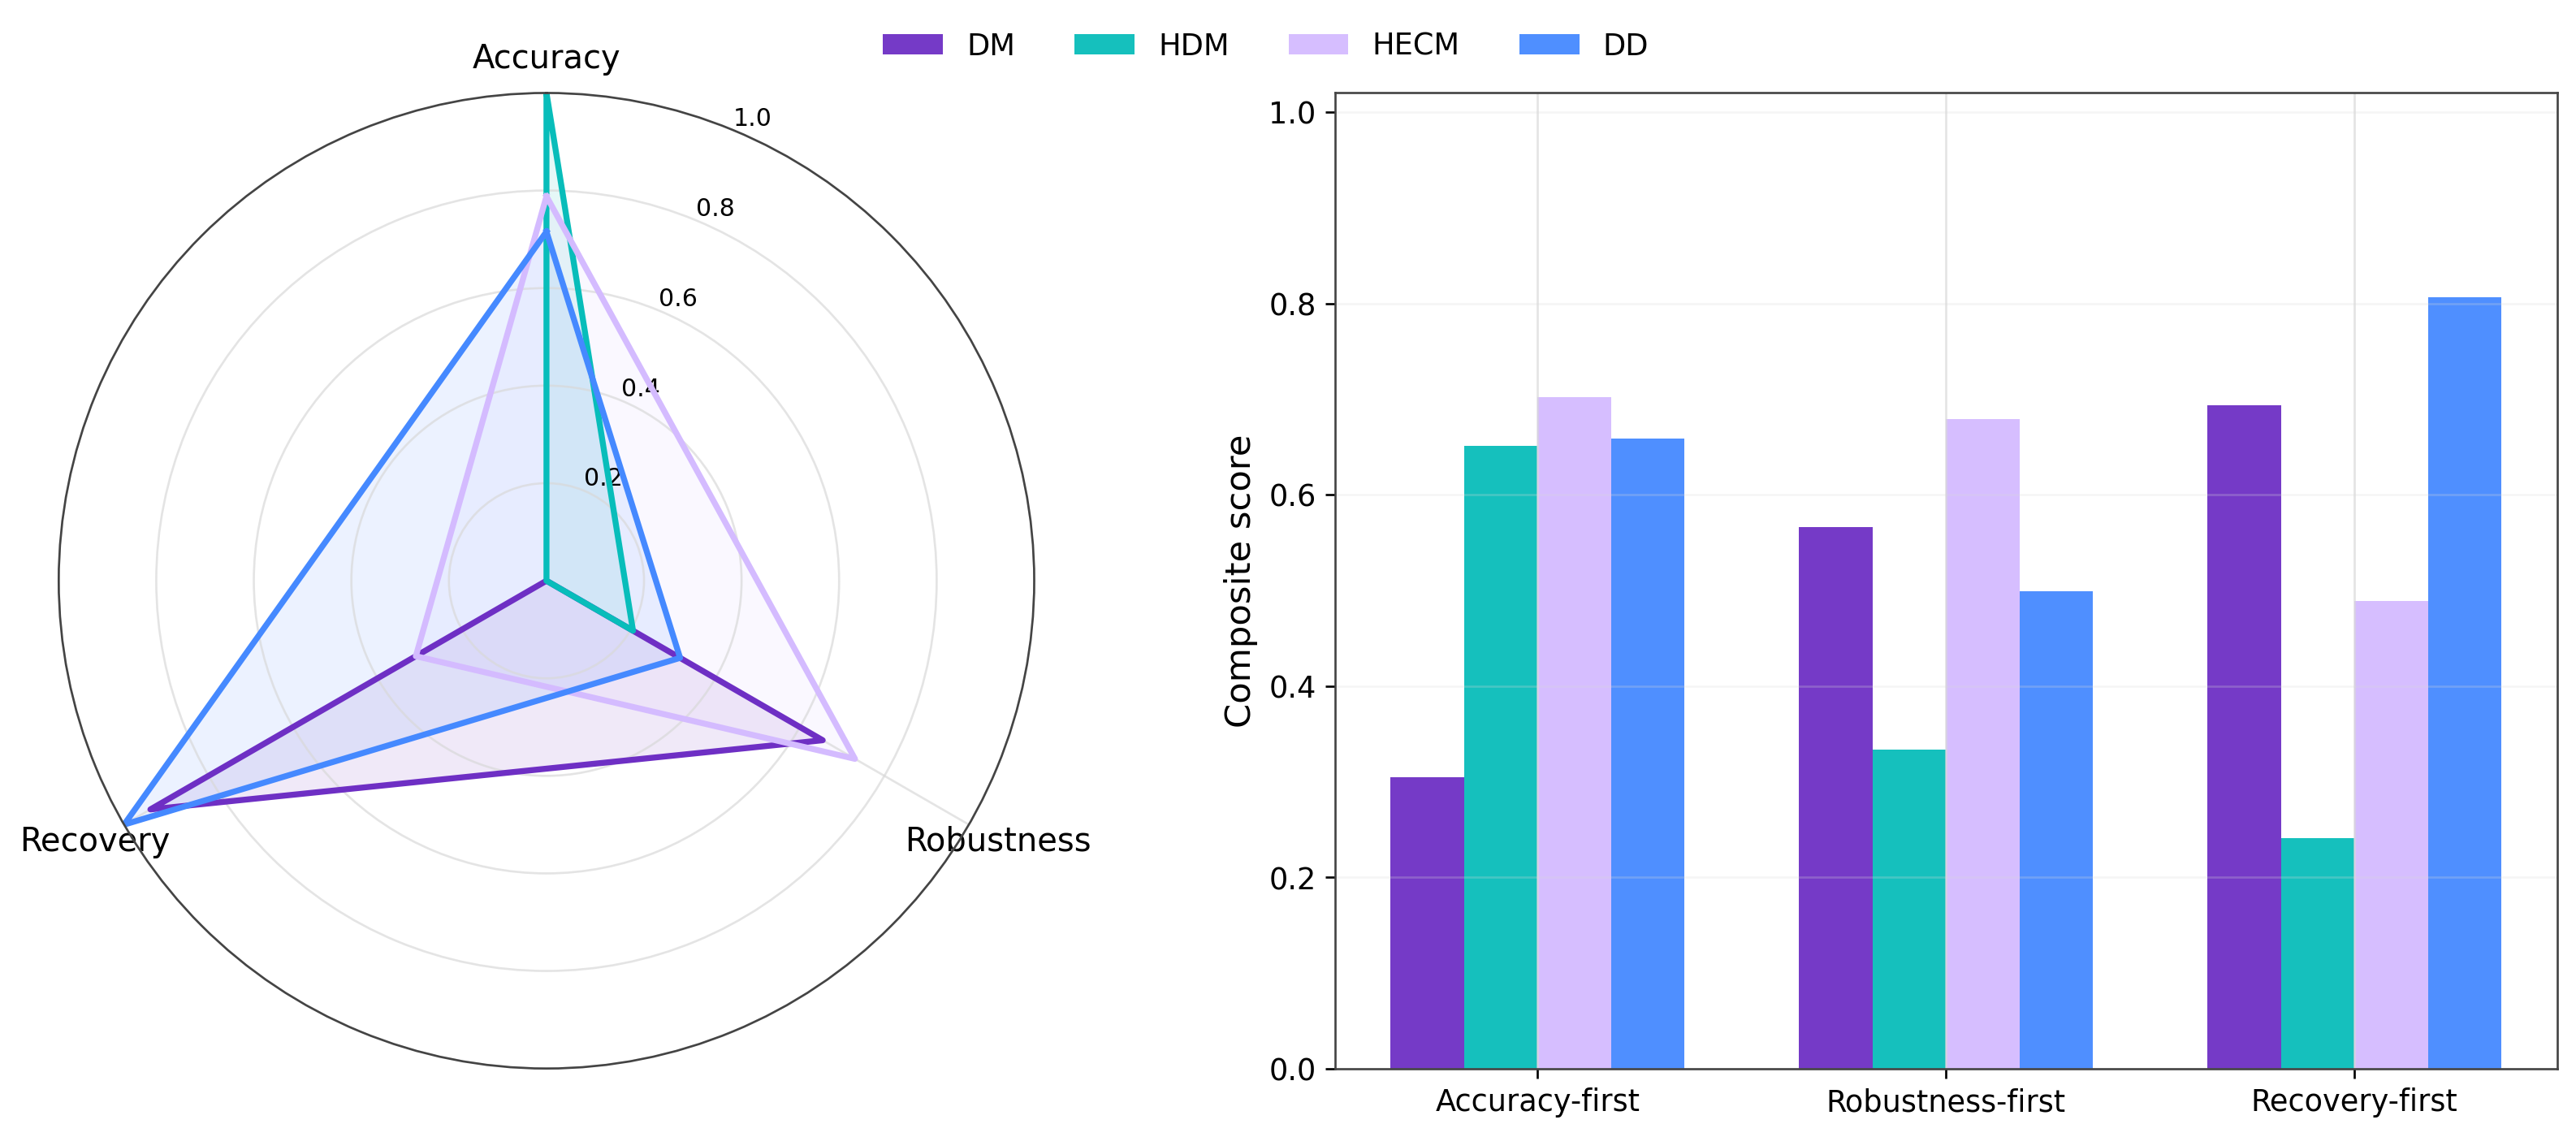
\includegraphics[width=\textwidth]{robustness_decision_synthesis.png}
    \caption{Decision-oriented synthesis from the robustness benchmark. This fits naturally into the dissertation because it already translates experimental results into estimator-selection guidance.}
    \label{fig:robustness_decision}
\end{figure}

\chapter{Embedded Artificial Intelligence for SOC and SOH Estimation on Microcontrollers}
\chapterrole{This chapter should integrate the embedded paper as the bridge from battery AI models to resource-constrained execution. It is the chapter in which the dissertation becomes explicitly about embedded implementation quality, not only about estimator behavior.}

\section{Core Contribution}
The embedded AI paper contributes the deployment path from floating-point sequence models toward practical MCU inference through pruning, quantization, and on-device KPI analysis. Within the dissertation, this chapter should establish that architecture design and embedded execution cannot be separated once the target application is a BMS.\autocite{paper2_embedded}

\section{Material to Reuse from the Paper}
\begin{itemize}[leftmargin=*]
\item the SOC/SOH model pipeline and streaming inference setup,
\item the pruning and quantization methodology,
\item the STM32-based measurement workflow,
\item Flash, RAM, and latency KPIs,
\item the trade-off analysis between resource savings and predictive quality.
\end{itemize}

\section{Dissertation-Specific Expansion}
To integrate smoothly into the dissertation, this chapter should emphasize:
\begin{itemize}[leftmargin=*]
\item how the embedded results depend on the robustness perspective introduced earlier,
\item how compression is constrained by estimator architecture and task structure,
\item how on-device execution metrics should influence model selection,
\item how the dev-board deployment relates to the broader BMS hardware ecosystem.
\end{itemize}

\begin{figure}[H]
    \centering
    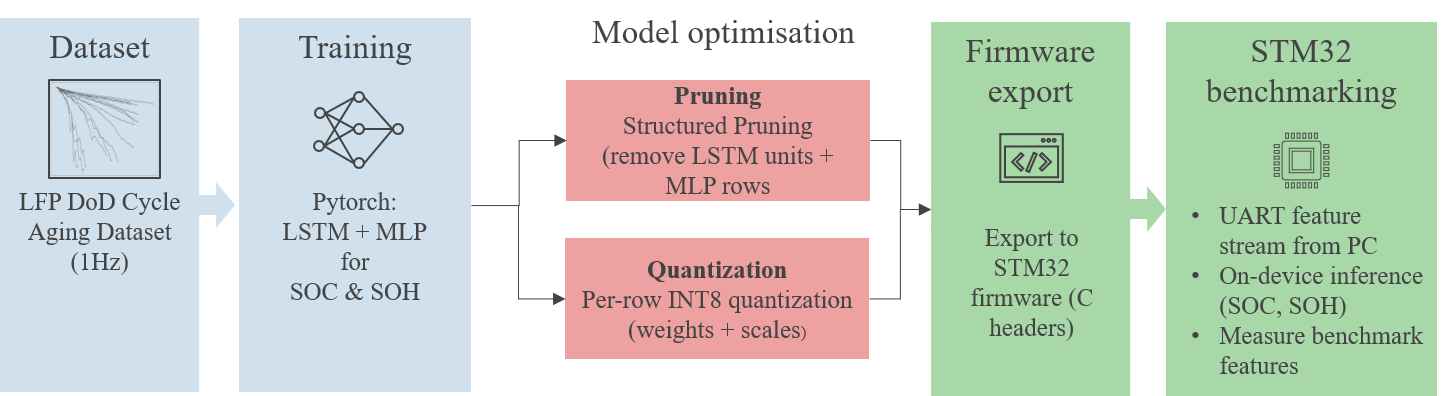
\includegraphics[width=0.95\textwidth]{embedded_pipeline.png}
    \caption{Embedded deployment pipeline reused as a dissertation anchor figure. This figure can connect software training, model export, and MCU execution in one visual narrative.}
    \label{fig:embedded_pipeline}
\end{figure}

\begin{figure}[H]
    \centering
    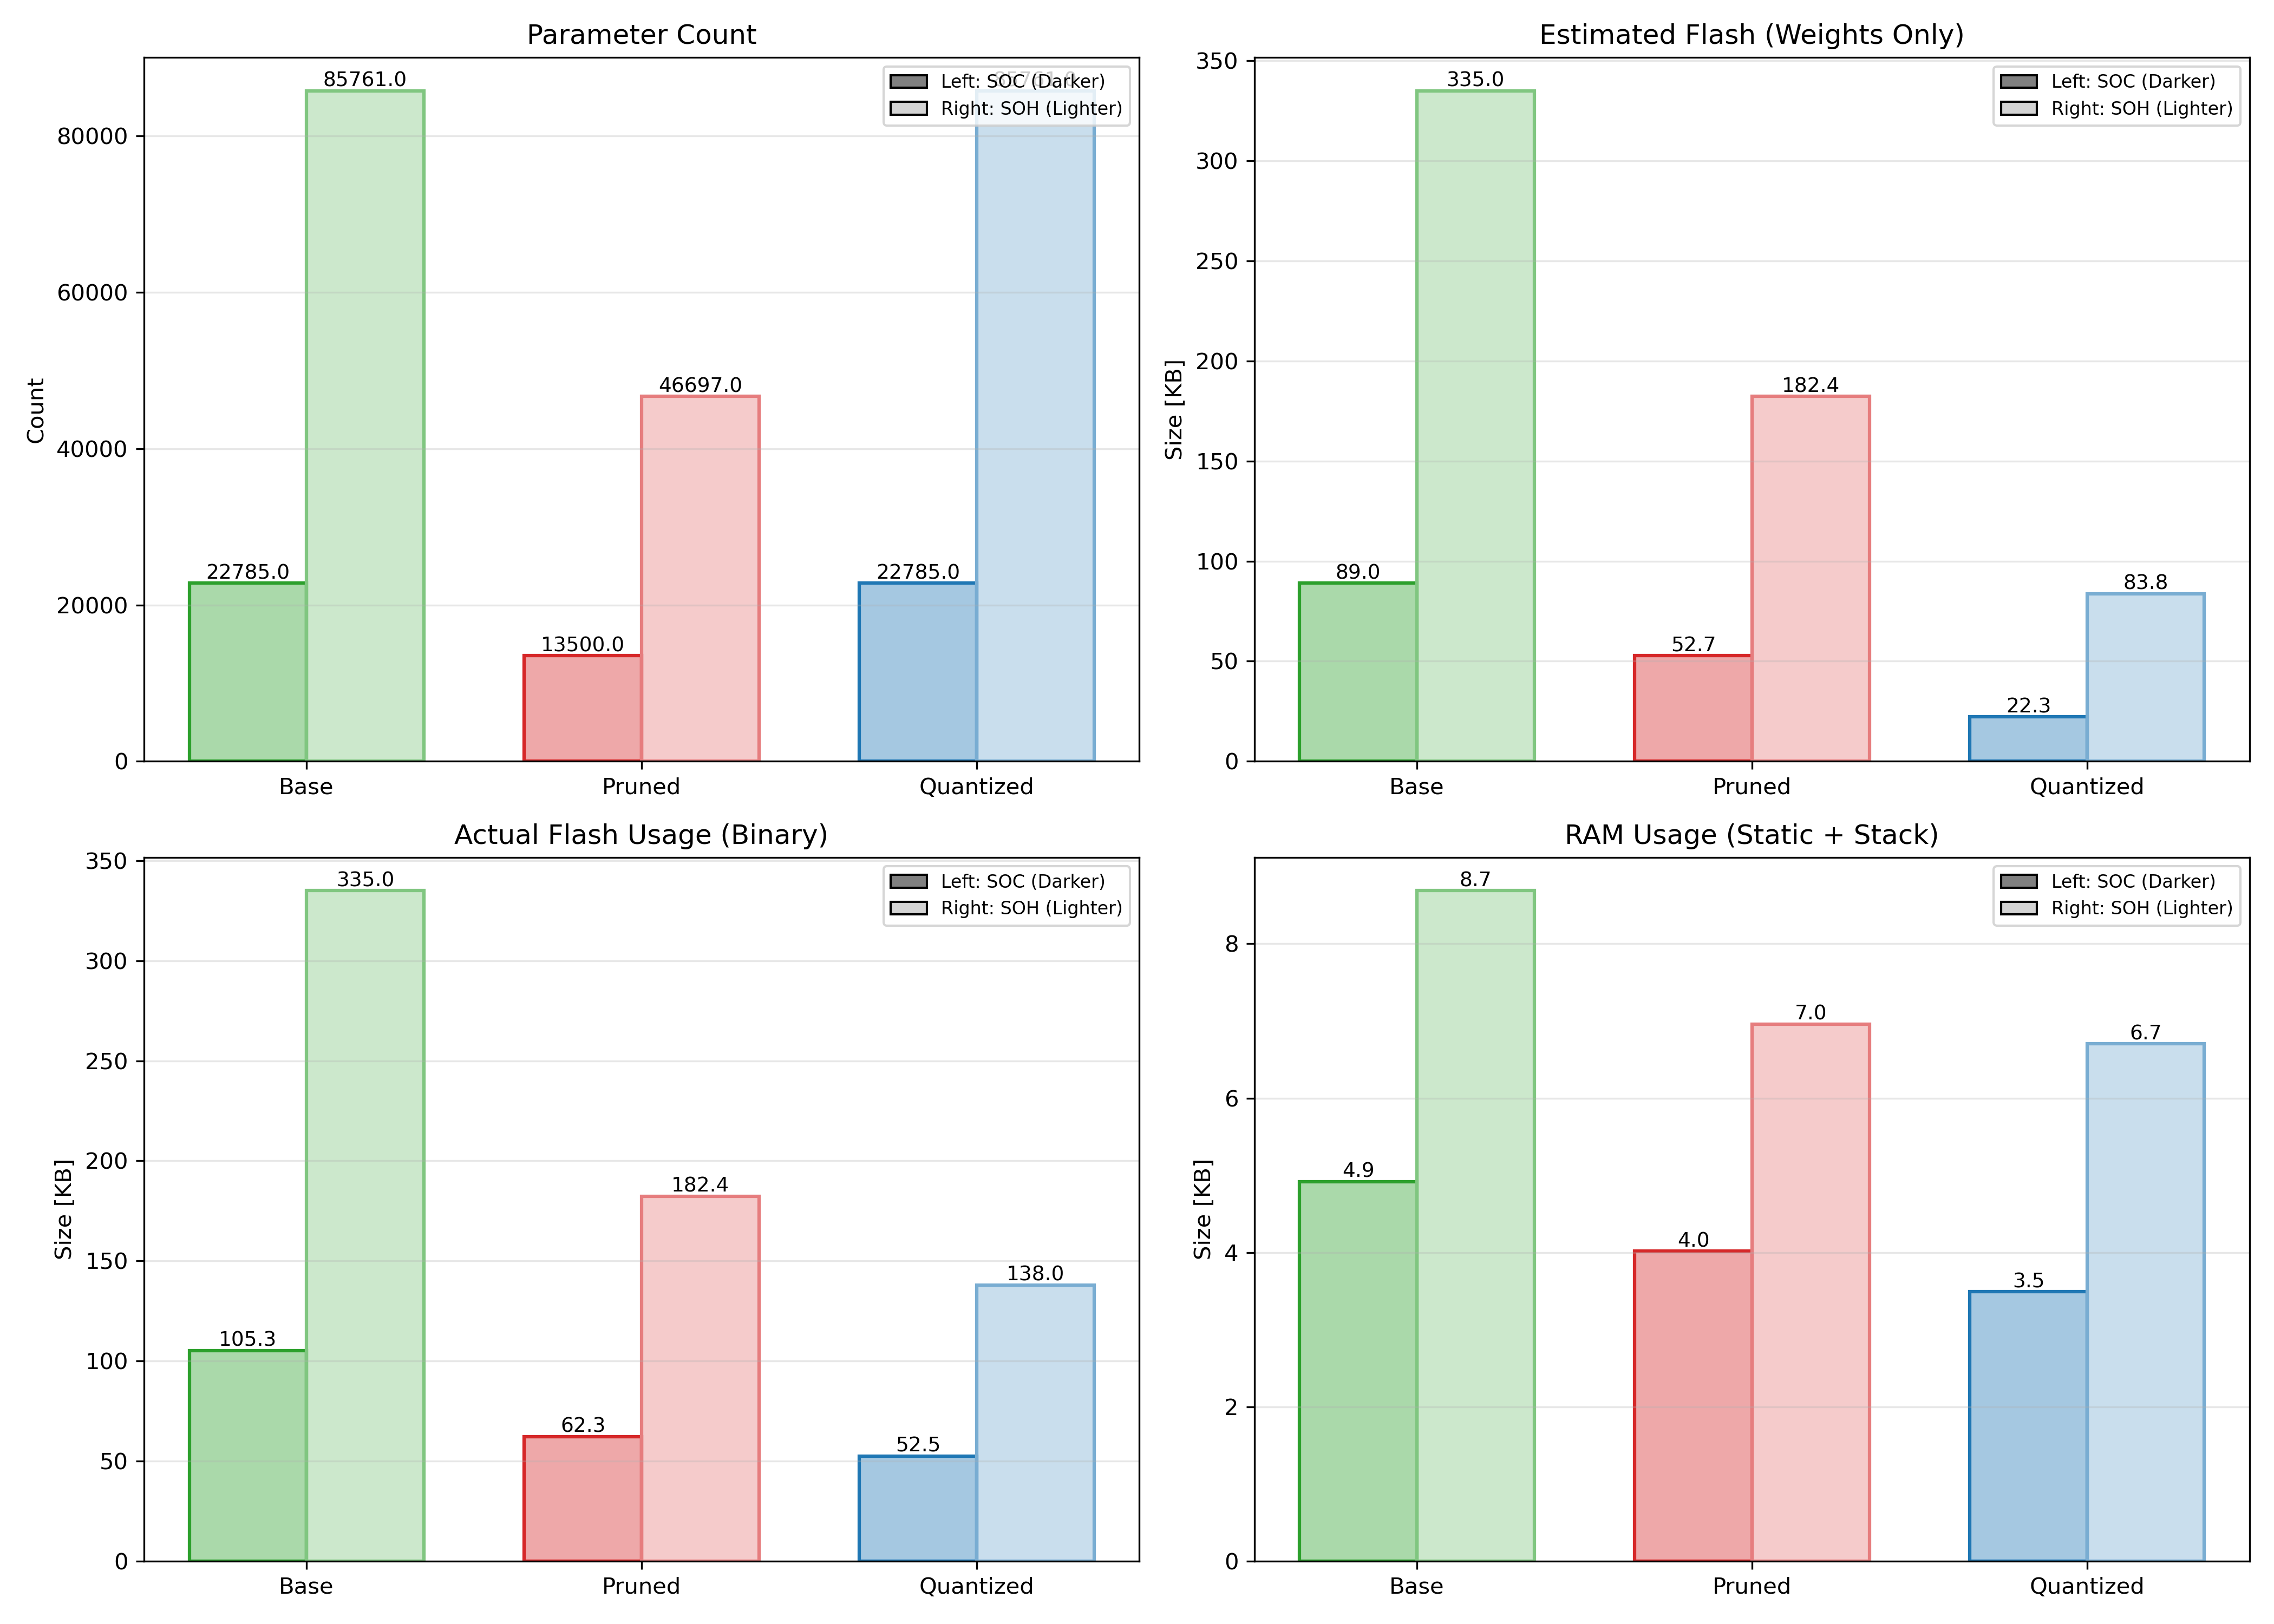
\includegraphics[width=0.95\textwidth]{embedded_model_sizes.png}
    \caption{Resource landscape for the embedded AI chapter. In the dissertation, this type of figure will help position resource efficiency as a first-class evaluation dimension rather than an appendix metric.}
    \label{fig:embedded_resources}
\end{figure}

\chapter{Planned Comparative Study on Pruning and Quantization Across Model Architectures}
\chapterrole{This planned chapter is the cleanest place to introduce the next paper you described. It should extend the current embedded results from one concrete pipeline toward a broader model-compression design framework.}

\section{Why This Chapter Matters}
The existing embedded paper already shows that pruning and quantization can be useful. The next logical step is to ask whether those gains hold equally across very different model families. This is where the dissertation can move beyond a single embedded case study and develop genuinely transferable design rules.

\section{Recommended Scope}
The planned comparison chapter should explicitly vary both architecture and compression strategy. A useful comparison matrix would likely include:
\begin{itemize}[leftmargin=*]
\item feed-forward or lightweight MLP baselines,
\item recurrent models such as GRU or LSTM,
\item hybrid models with explicit state or physics-based structure,
\item multiple pruning ratios and multiple quantization schemes,
\item shared embedded KPIs and task-specific accuracy metrics.
\end{itemize}

\begin{table}[H]
    \centering
    \caption{Proposed experiment matrix for the planned compression chapter.}
    \label{tab:planned_compression_matrix}
    \begin{tabularx}{\textwidth}{p{3.0cm}p{3.4cm}p{3.2cm}Y}
        \toprule
        Model family & Main task & Compression variables & Expected dissertation value \\
        \midrule
        MLP & SOH or static surrogate tasks & INT8, mixed precision, structured pruning & Simple low-cost baseline and reference point for interpretability and resource use. \\
        GRU / LSTM & Streaming SOC or SOH & hidden-size pruning, INT8 export, activation range analysis & Direct continuation of the current embedded AI work. \\
        Hybrid neural / physics-aware models & SOC correction or joint estimation & selective compression of neural sub-blocks & Useful for understanding whether hybrid structures compress differently from purely neural ones. \\
        Tiny deployment baselines & MCU-only inference & aggressive compression and latency-first tuning & Practical lower-bound reference for real BMS integration. \\
        \bottomrule
    \end{tabularx}
\end{table}

\begin{figure}[H]
    \centering
    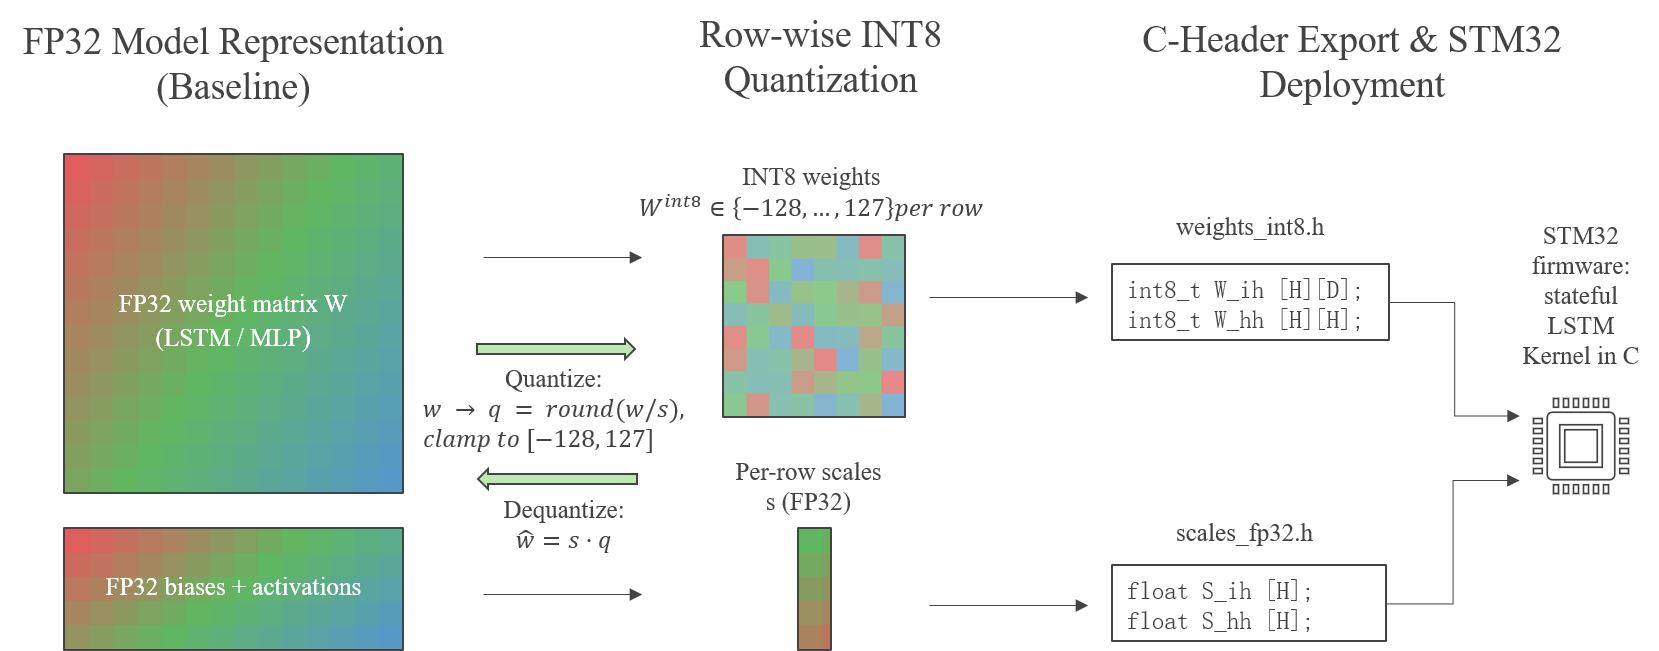
\includegraphics[width=0.92\textwidth]{embedded_quantization.png}
    \caption{Existing quantization schematic reused as the visual starting point for the planned architecture-comparison chapter.}
    \label{fig:planned_quantization}
\end{figure}

\section{How This Chapter Fits the Overall Thesis}
This future chapter should not be presented as an isolated extra paper. It is the natural continuation of the embedded story:
\begin{itemize}[leftmargin=*]
\item Chapter 5 asks how architectures represent ageing information.
\item Chapter 6 asks how estimator classes behave under disturbance.
\item Chapter 7 asks how one embedded pipeline behaves under compression.
\item Chapter 8 generalizes the compression question across architectures.
\end{itemize}

\chapter{Cross-Paper Synthesis and Design Guidelines}
\chapterrole{This synthesis chapter should make the dissertation more valuable than the sum of the included papers. It is the place where the three requirement dimensions are turned into practical design rules.}

\section{Integrated Design Perspective}
The dissertation should culminate in a design-oriented synthesis chapter rather than stop at paper-specific summaries. This chapter can explicitly state what the combined work teaches about choosing battery-AI methods under practical deployment constraints.

\section{Proposed Synthesis Matrix}
\begin{table}[H]
    \centering
    \caption{Proposed synthesis matrix that links dissertation chapters to the three central requirement dimensions.}
    \label{tab:synthesis_matrix}
    \begin{tabularx}{\textwidth}{p{3.8cm}p{2.7cm}p{2.7cm}Y}
        \toprule
        Dissertation contribution & Performance & Hardware / embedded & Implementation logic \\
        \midrule
        Neural ageing-estimation chapter & high relevance for representation quality & indirect relevance & strong relevance for architecture and feature design \\
        Robustness benchmark chapter & strongest relevance & medium relevance through sensing realism & strong relevance for evaluation methodology \\
        Embedded AI chapter & medium relevance & strongest relevance & strongest relevance for compression and deployment workflow \\
        Planned compression chapter & medium relevance & strongest relevance & strongest relevance for model-hardware co-design \\
        Hardware ecosystem chapter & indirect relevance & strongest relevance & medium relevance through system integration \\
        \bottomrule
    \end{tabularx}
\end{table}

\section{Candidate Final Design Rules}
This final synthesis chapter is the right location for concise design rules such as:
\begin{itemize}[leftmargin=*]
\item do not choose estimators by clean-condition accuracy alone,
\item evaluate robustness before optimizing for compression,
\item treat quantization and pruning as architecture-dependent design choices,
\item separate dataset quality, estimator quality, and embedded execution quality,
\item connect all algorithmic claims to a credible hardware and validation chain.
\end{itemize}

\section{Why the Dissertation Benefits from This Structure}
This organization allows each paper to keep its own technical identity while avoiding three common cumulative-dissertation problems:
\begin{itemize}[leftmargin=*]
\item repeated background across chapters,
\item unclear progression from one publication to the next,
\item missing synthesis beyond already published paper conclusions.
\end{itemize}

\chapter{Conclusion and Outlook}
\chapterrole{The concluding chapter should close the dissertation at the synthesis level rather than only repeat chapter summaries.}

The final dissertation should conclude that deployment-oriented battery AI emerges only when model design, robustness, embedded execution, and hardware integration are treated as one linked problem. The current structure already supports that conclusion by giving each paper a clear role inside a broader argument.

\section{Immediate Next Writing Steps}
\begin{itemize}[leftmargin=*]
\item decide whether the final dissertation language will remain fully English,
\item finalize the chapter order and the chapter titles,
\item decide how much of each paper is reused almost verbatim and how much is rewritten,
\item collect the available hardware material for the custom BMS chapter,
\item define the concrete experiment matrix for the planned compression paper.
\end{itemize}

\section{Likely Final Contribution Statement}
The likely final contribution of the dissertation is a deployment-oriented framework for AI-enabled battery management systems that spans:
\begin{itemize}[leftmargin=*]
\item neural ageing estimation,
\item robustness-oriented estimator evaluation,
\item resource-constrained embedded inference,
\item model-compression co-design,
\item and practical hardware integration.
\end{itemize}

\printbibliography

\appendix
\chapter{Reserved Appendix Space}
This appendix is intentionally left as a placeholder for supplementary tables, additional hardware documentation, experiment matrices, and publication-specific material that should not interrupt the flow of the main dissertation.

\end{document}
